\section{Model assessment}\label{subsec:Cost}
\subsection{The Rate of True-Positve - ROC Curve}\label{subsec:AUC}
A \ac{ROC} curve is a tool used to measure and visualize a binary classifiers' ability 
to predict trends. In figure \ref{fig:ROC} I have plotted an illustration of a \ac{ROC} curve.
The curve is plotted on an x-, y-axis where the x-axis represents 
false-positive rates and the y-axis represents true-positive. The different values 
for the curve are the rate of true positives with different thresholds, i.e. 
the value deciding whether an event is 1 or 0, signal or background. If a classifier 
has learned nothing and is simply guessing, the \ac{ROC} curve will be a linear curve 
going from 0 to 1. This line is often drawn in \ac{ROC} curve. The better the 
classifier is, the higher the \ac{ROC} curve will bend towards the upper-left corner of the 
graph. The worse it is, the more it will bend to the lower right corner. 
\\
A metric often used to measure a classifiers' ability create an output which effectively 
separates two categories, is the \ac{AUC}. The higher the area, the larger the separation. 
An ideal classifier which perfectly separates two categories will achieve a \ac{AUC} of 1.
A classifier which simply guesses, will achieve an \ac{AUC} of 0.5. Both this cases assume 
an equal weighting of both signal and background. 
\begin{figure}
    \centering
    \makebox[0.75\linewidth][c]{%
    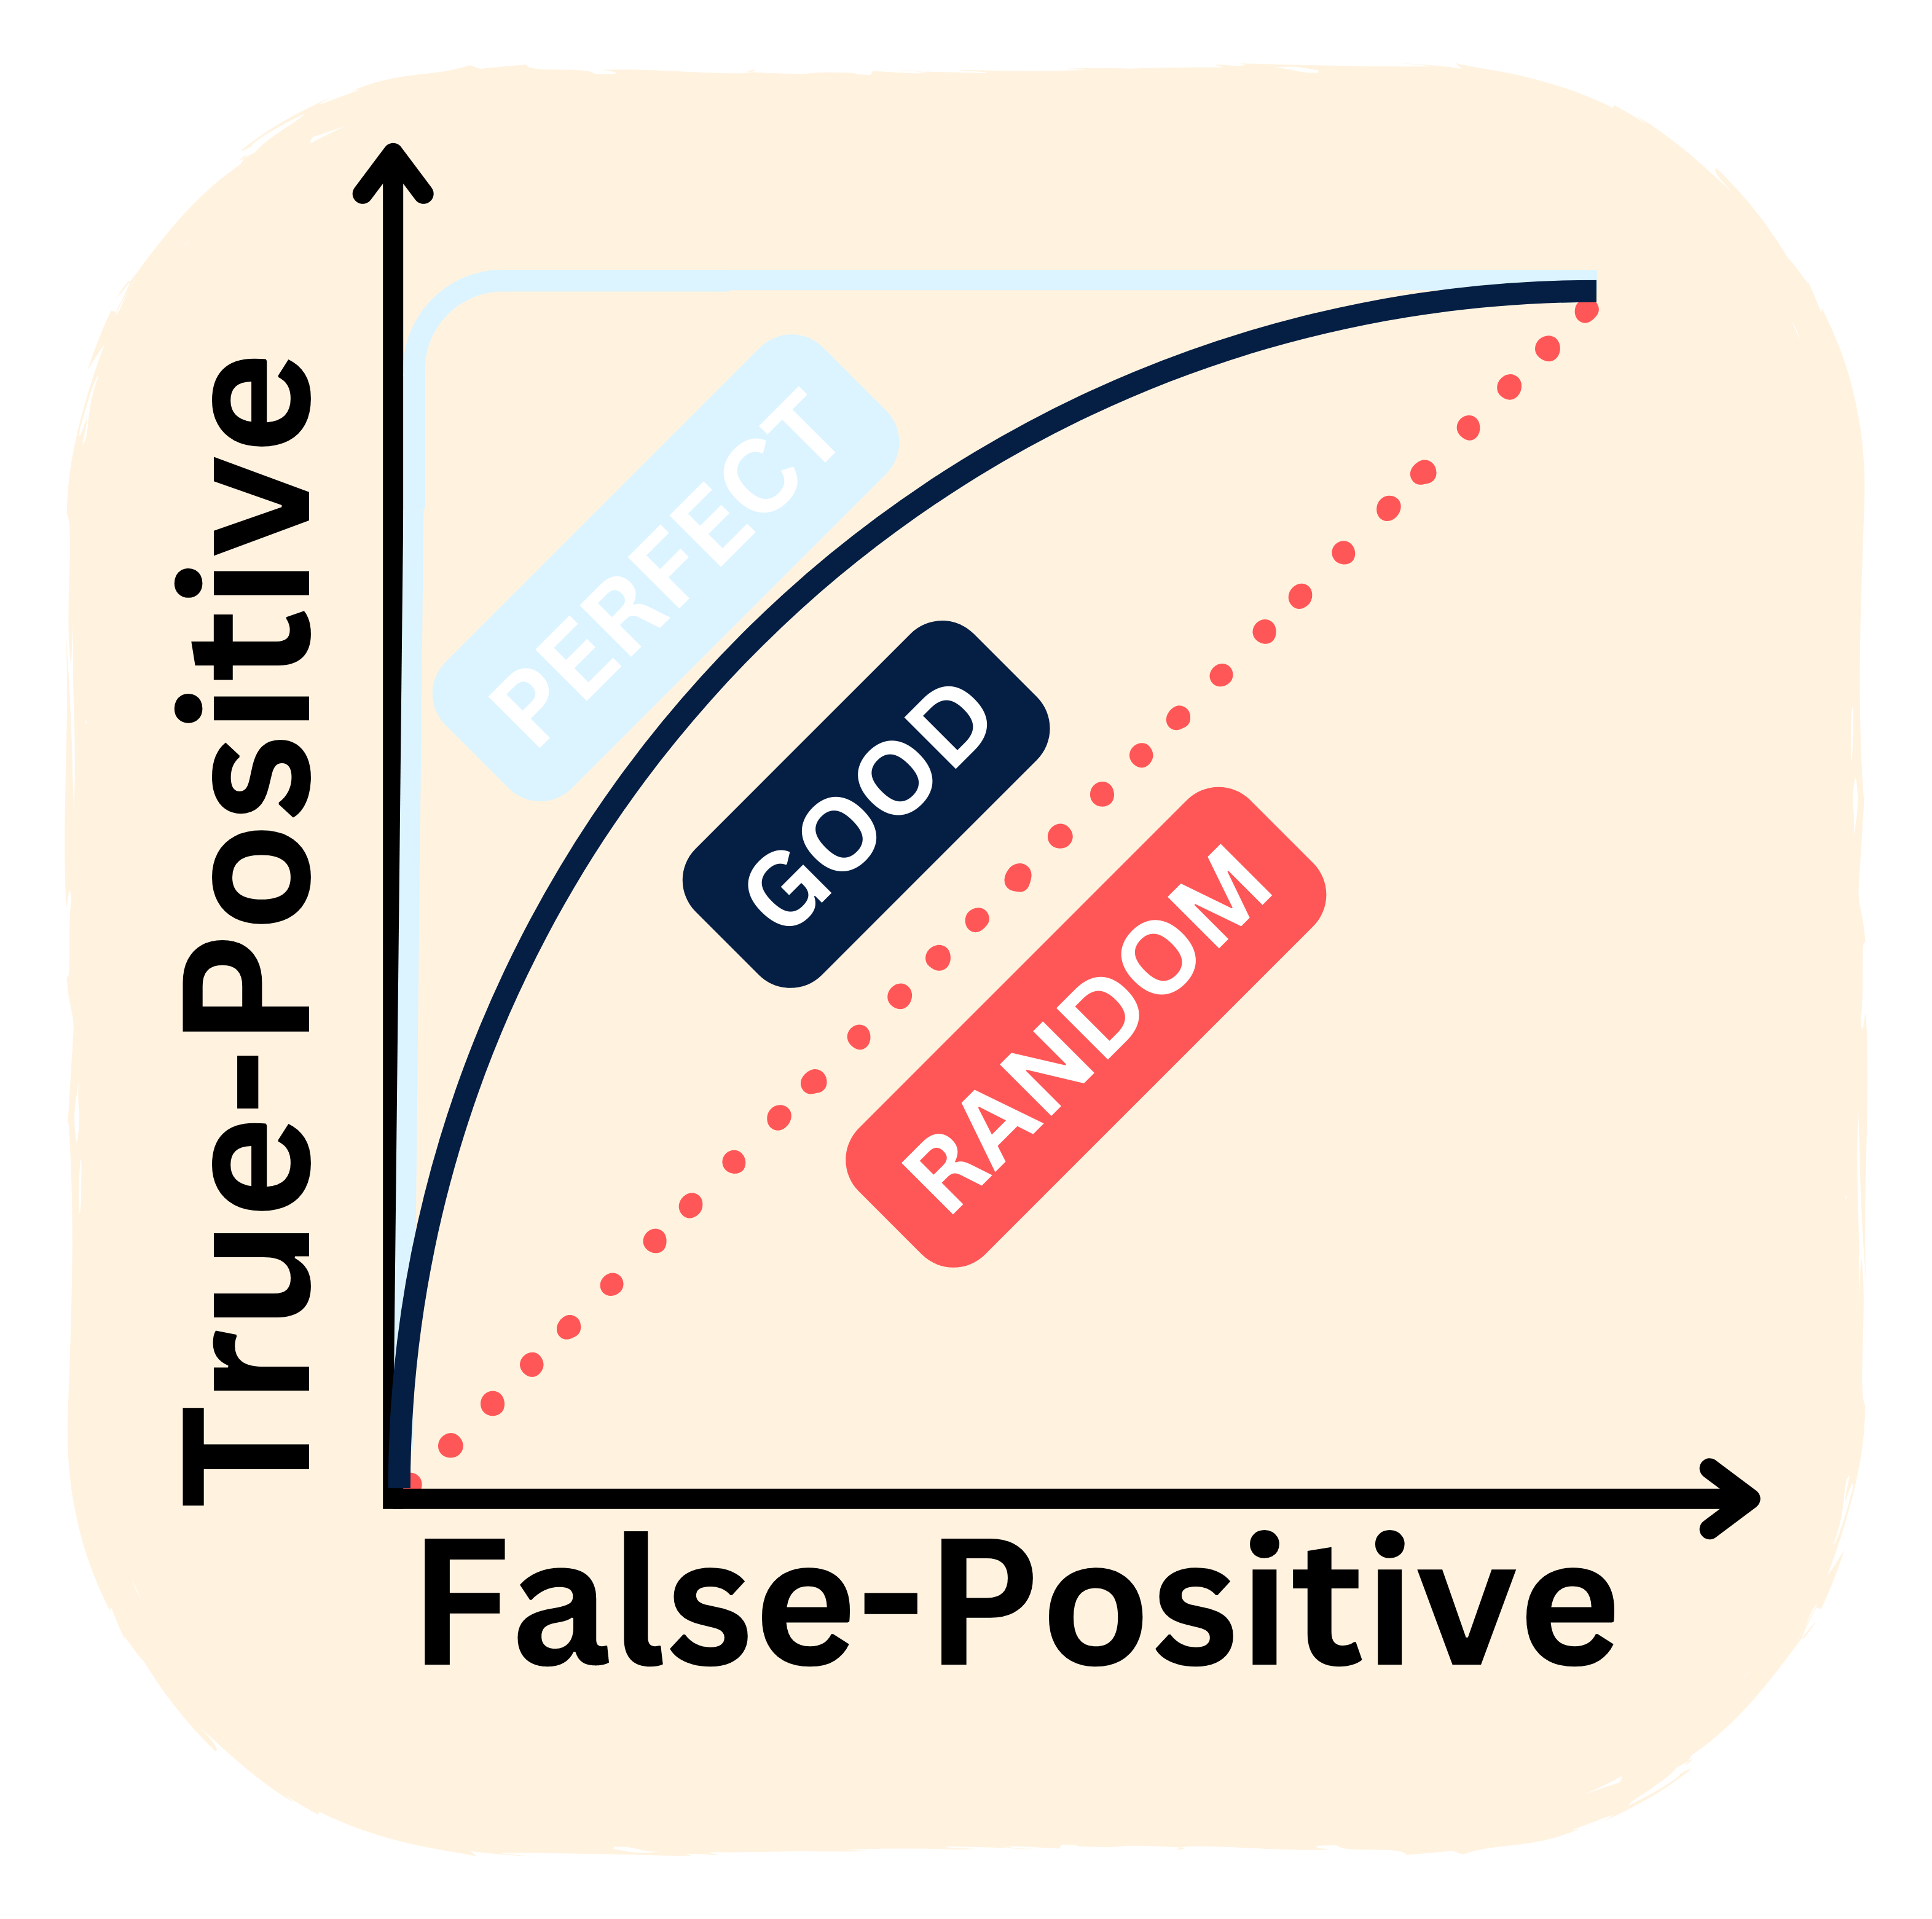
\includegraphics[width=0.45\textwidth]{Figures/Illustrations/True-Positive.png}
    }
    \caption{An illustration of a ROC curve.}
    \label{fig:ROC}
\end{figure}
\subsection{Statistical Assessment - Discovery $\&$ Exclusion}\label{subsec:Sensitivity}
The statistical aspect of the analysis will not be of focus in this analysis, nonetheless there are 
some expressions which would be helpful to define. Let us assume that we expect to see no new physics in the collision
data, we can call this hypothesis the b(background)-hypothesis. To expect no new physics, is not the same as expecting no 
deviation between \ac{SM} simulations and experiment. We still assume a statistical uncertainty, or noise to effect the simulations which 
will lead to some deviations. If these deviations are random, we can assume that the noise can be described as sampling from a Gaussian distribution 
(which is a good approximation for large statistics), which has a mean of 0 and a standard deviation equal to $\sqrt{b}$, where b is 
the number of \ac{SM} simulations. Using this assumption, we can state that the higher the deviation between the two, i.e. the further away 
from the mean, the less likely such a deviation is explained by our b-hypothesis. Given a large enough deviation, we can even 
define the hypothesis as rejected.
\\
We measure the deviation between the observed collision data and the simulated \ac{SM} data in units of significance, Z. 
For a given signal region with $n_{obs}$ events of measured collision data and b simulated \ac{SM} data, we define
the significance of a deviation as
\begin{align}
Z=\sqrt{2\left[n_{\text {obs }} \ln \frac{n_{\text {obs }}}{b}-n_{\mathrm{obs}}+b\right]} \text { or } 
Z=\sqrt{2\left[(s+b) \ln \left(1+\frac{s}{b}\right)-s\right]}, 
\end{align}
where we have defined the signal, s as $s = n_{obs} - b$. In the case of large statistics ($b>>s$), we can write Z 
as 
\begin{align}\label{eq:Z}
    Z=\frac{n_{o b s}-b}{\sqrt{b}} = \frac{s}{\sqrt{b}}.
\end{align}
By studying equation \ref{eq:Z} we observe that the significance of a deviation, is simply the signal measured in units of standard
deviation of the Gaussian distribution. In physics, one often deems the results a discovery, or the b-hypothesis as rejected if Z is 
larger than 5. 
\\
In the case we are not intrested in discovering physics, but simple to measure the sensitivity of a model, we can also use 
significance. In this case we do not have $n_{obs}$. Instead we simply define s as the number of events for the simulated signal 
inside the signal region. This number would be spesific for each mass combination and will be a measure for how sensitive 
the model is for that exact combination. In physics, we define a model as sufficiently sensitive, if it is able to achieve a 
significance of 1.64. This number is chosen based on its relation to the b-hypothesis. A significance of 1.64, equals the 
distance from the mean of the Gaussian distibution which sums to an area of 0.90 (see figure \ref{fig:ConfInt}). There are many ways to inteprate this. A layman 
intepration (which is sufficient for this theisis), is that given the b-hypothesis is true, there is a $90\%$ probability that we will 
measure a signal which produces a significance of less than 1.64. Therefore, there is only a $10\%$ probability that the b-hypothesis
can explain the deviation. For more information on significance and discovery in physics the reader is reffered to the slides \cite{magnar}.
\begin{figure}
    \centering
    \makebox[0.8\linewidth][c]{%
    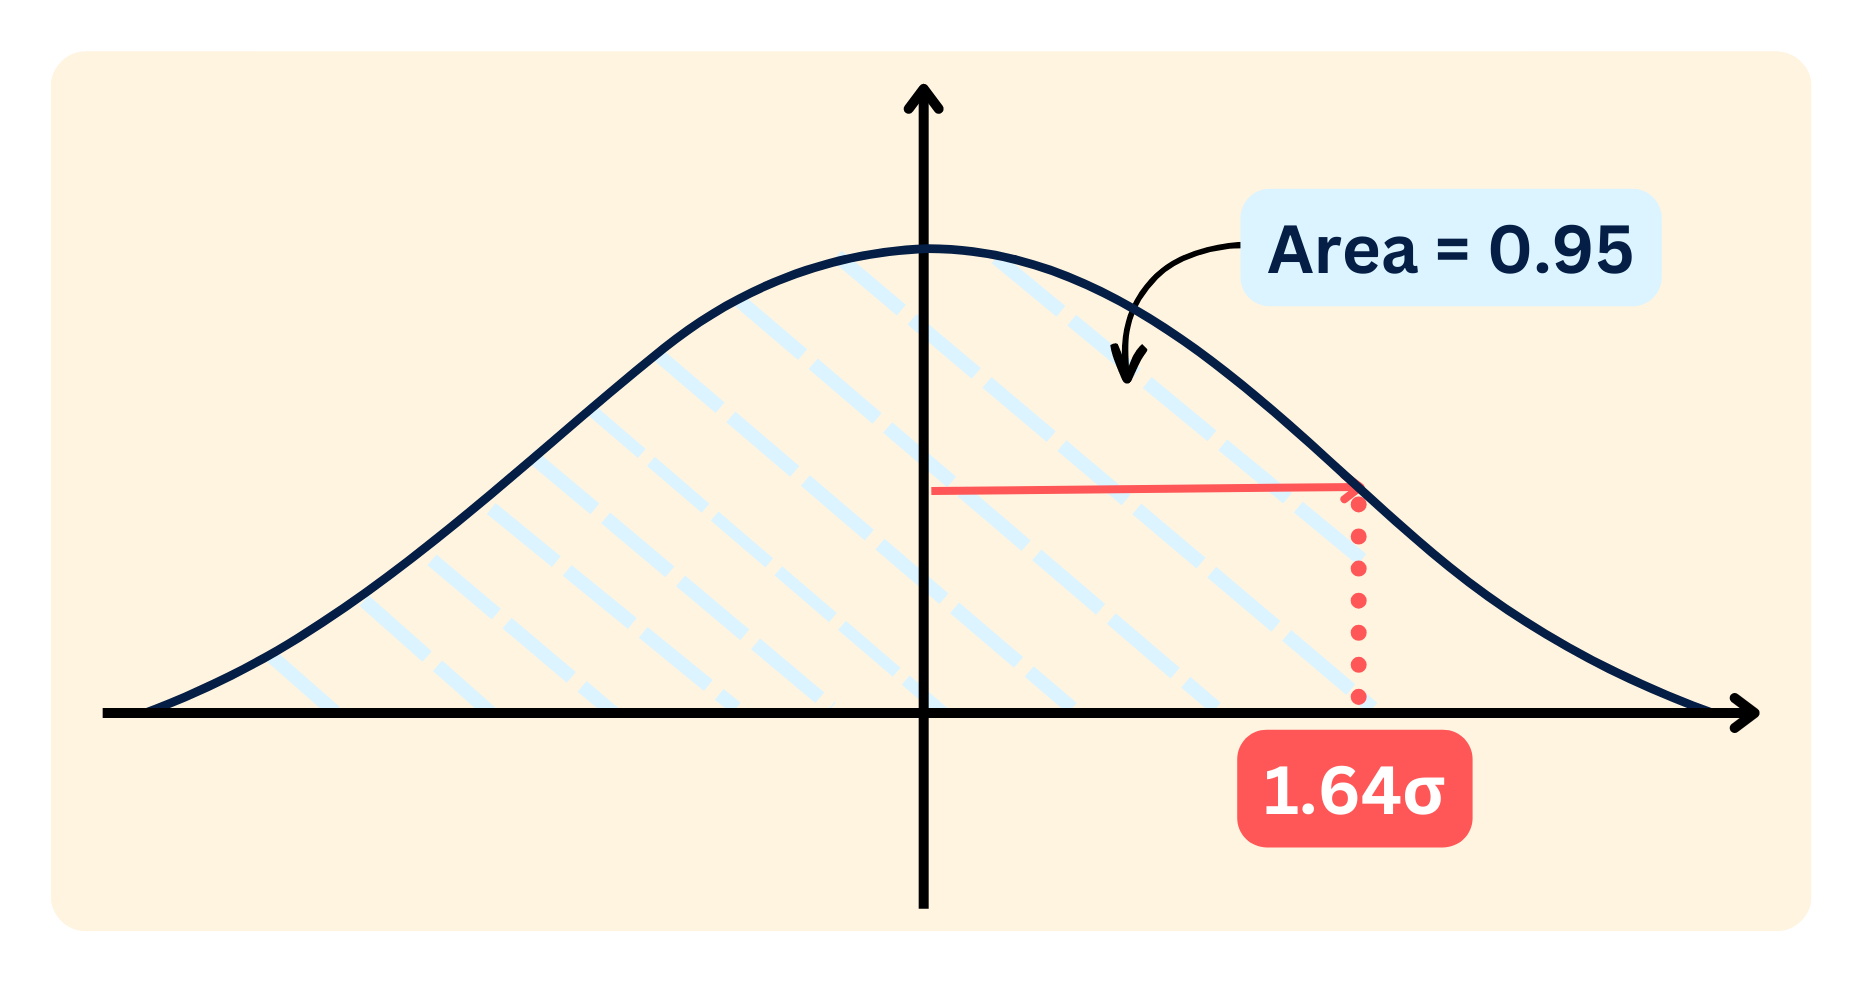
\includegraphics[width=0.45\textwidth]{Figures/Illustrations/ConfInt.png}
    }
    \caption{An illustration of a Gaussian distibution and the area under the curve defined by a significance equal to 1.64.}
    \label{fig:ConfInt}
\end{figure}
ADD SECTION ON UNCERTAINTY AND THE FORMULA ROOT USES
% \subsection{Confidence Interval}
% By defining the signal as the deviation between the simmulated and measured data, we risk missintepreting noise in either the 
% experiment or the simmulations, as signal. If we assume that said noise is sampled from a random Gaussian distibution centered around 
% zero, the significance takes on another meaning. If start by assuming that any deviation is rooted in noise, than we can inteprate the significance
% as the measure of how likely this assumtion is to be true. The larger the significance, the more likely that the deviation is not described 
% by noise sampled from a gaussion distribution, but instead by something not random at all, new physics. Obviously the most likely deviation 
% given the noise is approximated by a Gaussian distribution, is 0. Whereas the larger deviation/signal we find, and therefore the larger the significance 
% the less likly the hypothesis of no new physics. 
% (REWRITE THISNSECTION)
% \\
% The threshold for what is deemed a sufficient significance is not clearly defined, and is instead a matter of field. In this analysis, and generally 
% in the field of physics, a significane of 1.64 is defined as a sufficient sensitivity to be able to exclude a theory. Given the assumption of Gaussian
% distributed noise, a significance of 1.64 is ecuivilant to a $90\%$ confidence interval. This means that if the experiment was repeated, then there would 
% $10\%$ probability that the result would not be repeated, and that the hypothsis still holds true.

% \ac{AUC} is a very good measure of how separated the distribution for signal and background are 
% for a feature. In the search for new physics, features with large separation between signal and background
% are incredibly helpful, but not the end goal. The final result in the search for new physics is the discovery 
% of a significant deviation between the \ac{SM} and experiment.